%             
% Hall D Note
% 
\documentclass[12pt]{article}


\usepackage{color}

% ===    Set a true/false value for PDF hyper marks  

\newif\ifhyprf
%\hyprffalse   
\hyprftrue

\RequirePackage{ifpdf}
  
\ifpdf
    \pdfoutput=1        % we are running PDFLaTeX
    \pdftrue
\else
    \pdffalse           % we are not running PDFLaTeX
\fi

\ifpdf
  \pdfcompresslevel=9
  \usepackage[pdftex]{graphicx}
%  \usepackage{thumbpdf}
  \definecolor{rltred}{rgb}{0.75,0,0}
  \definecolor{rltgreen}{rgb}{0,0.3,0}
  \definecolor{rltblue}{rgb}{0,0,0.75}
  \definecolor{rltdarkgreen}{rgb}{0.1,0.6,0.1}
  \ifhyprf
     \usepackage[pdftex,
         colorlinks=true,
         urlcolor=rltblue,       % \href{...}{...} external (URL)
         filecolor=rltgreen,     % \href{...} local file
         linkcolor=rltred,       % \ref{...} and \pageref{...}
         citecolor=rltdarkgreen, % citations
         pagebackref,
         pdfpagemode=None,
         pdftitle={Civil Reference Concepts for BDX},
         pdfauthor={many},
         pdfsubject={Civil Reference Concepts for BDX},
         pdfkeywords={JLab Beam Dump Experiment}]{hyperref}
  \fi
  \usepackage{pdfcolmk}
  \DeclareGraphicsExtensions{.pdf,.png,.jpg}
\else
  \usepackage{graphicx}
  \DeclareGraphicsExtensions{.eps,.epsi,.ps,.eps.gz,.epsi.gz,.ps.gz}
\fi

\setlength{\textwidth}{6.0in}
%\setlength{\textheight}{9.5in}
\setlength{\textheight}{8.75in}
\setlength{\evensidemargin}{0.25in}
\setlength{\oddsidemargin}{0.25in}
\setlength{\topmargin}{-0.25in}
\setlength{\footskip}{0.25in}
%\setlength{\parindent}{0pt}
%\setlength{\parskip}{0in}
\usepackage{graphicx,lscape,rotating}
\pagenumbering{arabic}
%\input epsf
\usepackage[utf8]{inputenc}

\begin{document}

\begin{flushright}
GlueX-doc-XXXX\\
github: eltonssmith/reports/CPP\_PID\_systematics\\
February 16, 2022
\end{flushright}



%\pagestyle{myheadings}
%\markright{BDX-NOTE-2015-002}

%%%%%%%%%%%%%%%%%%%%%%%%%%%%%%%%%  TITLE %%%%%%%%%%%%%%%%%%%%%%%%%%%%%%%%
\begin{center}
{\Large \bf Toy Model for PID systematics in CPP}\\*[0.5cm]
\end{center}
%%%%%%%%%%%%%%%%%%%%%%%%%%%%%%%  AUTHORS %%%%%%%%%%%%%%%%%%%%%%%%%%%%%%%% 

\begin{center}   
{\sc  E.S. Smith}\\  
\end{center}

%\tableofcontents

\section{Introduction}
We are in the process of clarifying the requirements for the multi-variate analysis (MVA) that will be used to determine the number
of $\pi^+\pi^-$ events in the data sample collected by the CPP experiment \cite{CPPexp}.  The pion pairs will be collected along with 
a large number of Bethe-Heitler $\mu^+\mu^-$ events that are produced with 10$\times$ the cross section. The ratio of cross sections is 
denoted by $\beta\approx 10$. In this sample dominated by muon pairs, we must determine the number of pions with high precision
and, at the same time, have a high rejection of muons. This is the goal of the MVA. 

The purpose of the present study is to provide guidelines for the requirements of the MVA that achieve the goals of the experiment. In Fig.\,\ref{fig:Proposal_Table2} 
we reproduce Table 2 of the experimental proposal, which contains a summary of the error budget for the experiment. CPP aims to determine
the $\pi^+\pi^-$ Primakoff cross section with a precision of 1.5\%. This uncertainty is dominated by contributions other than the $\pi/\mu$ 
particle-identification (PID) analysis that is the focus of this note. We propose that we limit all non-dominant contributions to the error budget,
such as this one, to be less than 0.5\%. Added in quadrature, this would increase the overall uncertainty to only 1.58\%. 

\begin{figure}[tbph]
\begin{center}
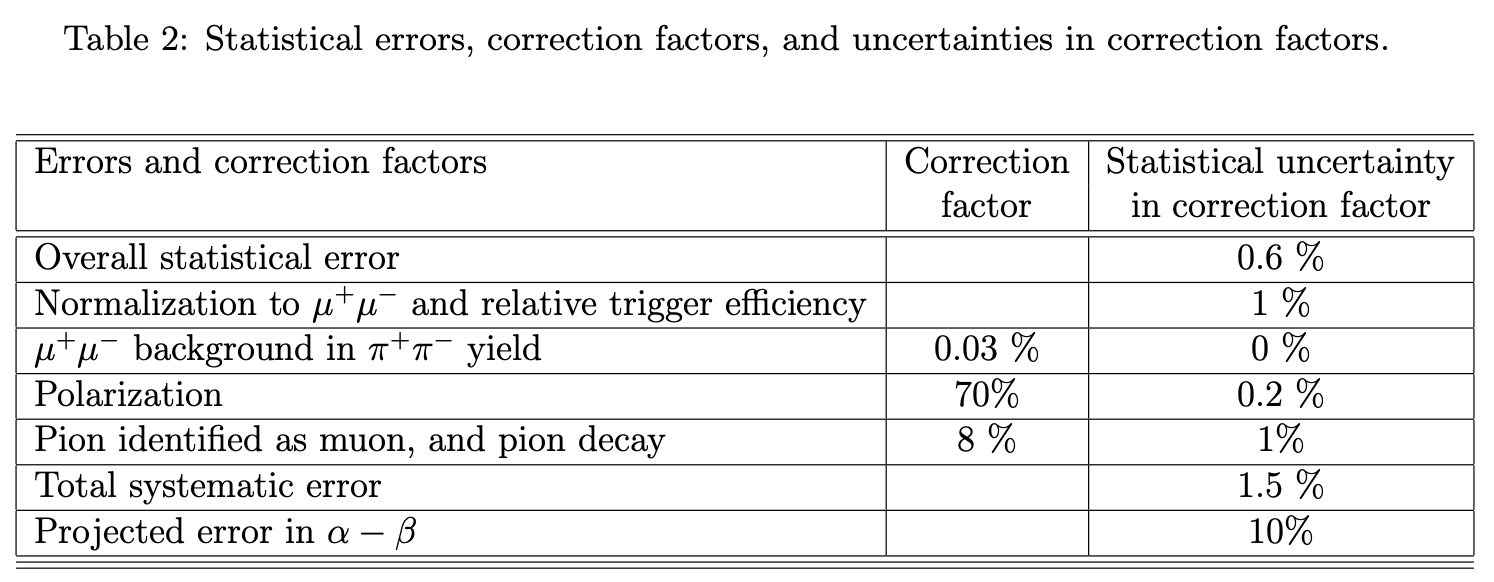
\includegraphics[height=6cm,clip=true]{Proposal_Table2}
\caption{Table 2 from the CPP Proposal \cite{CPPexp}. The goal of the experiment is to determine the Primakoff cross section with
an accuracy of 1.5\%. At the time of the proposal, the main contributors to the error budget were the overall statistical uncertainty, the absolute
normalization and the systematic uncertainty from pions identified as muons. The present study addresses a non-dominant systematic of 
$\pi/\mu$ particle identification.
\label{fig:Proposal_Table2}}
\end{center}
\end{figure} 

\section{Toy model}
We present a toy model for the MVA in order to gain insight into relevant dependencies that may contribute to the systematic uncertainty. 



\section{Toy model for PID systematics}
\begin{eqnarray}
N_m & = & \epsilon_\pi N_\pi + \epsilon_\mu N_\mu \\
N_\pi^m & = & {N_m - \epsilon_\mu N_\mu \over \epsilon_\pi}
\end{eqnarray}
Take
\begin{eqnarray}      
N_\mu & = & \beta N_\pi \\
N_\pi^m & = & {N_m - \epsilon_\mu \beta N_\pi \over \epsilon_\pi}
\end{eqnarray}
Since $\epsilon_\mu \le 10^{-3}$ (small), substitute $N_\pi \sim N_m/\epsilon_\pi$ in the second term.
\begin{eqnarray}
N_\pi^m & = & \left(N_m \over \epsilon_\pi \right) \left(1 - { \beta \over \epsilon_\pi} \epsilon_\mu \right)
\end{eqnarray}
The uncertainties in $N_\pi^m$ due to $\epsilon_\pi$ and $\epsilon_\mu$ are
\begin{eqnarray}
\delta N_\pi^m \over N_\pi^m & = & {\delta \epsilon_\pi \over \epsilon_\pi} \left( 1 + {\epsilon_\mu \beta \over \epsilon_\pi} \right)
\approx {\delta \epsilon_\pi \over \epsilon_\pi}
\end{eqnarray}
and
\begin{eqnarray}
\delta N_\pi^m \over N_\pi^m & = & {\beta \over \epsilon_\pi} \delta \epsilon_\mu 
\end{eqnarray}

\begin{figure}[tbph]
\begin{center}
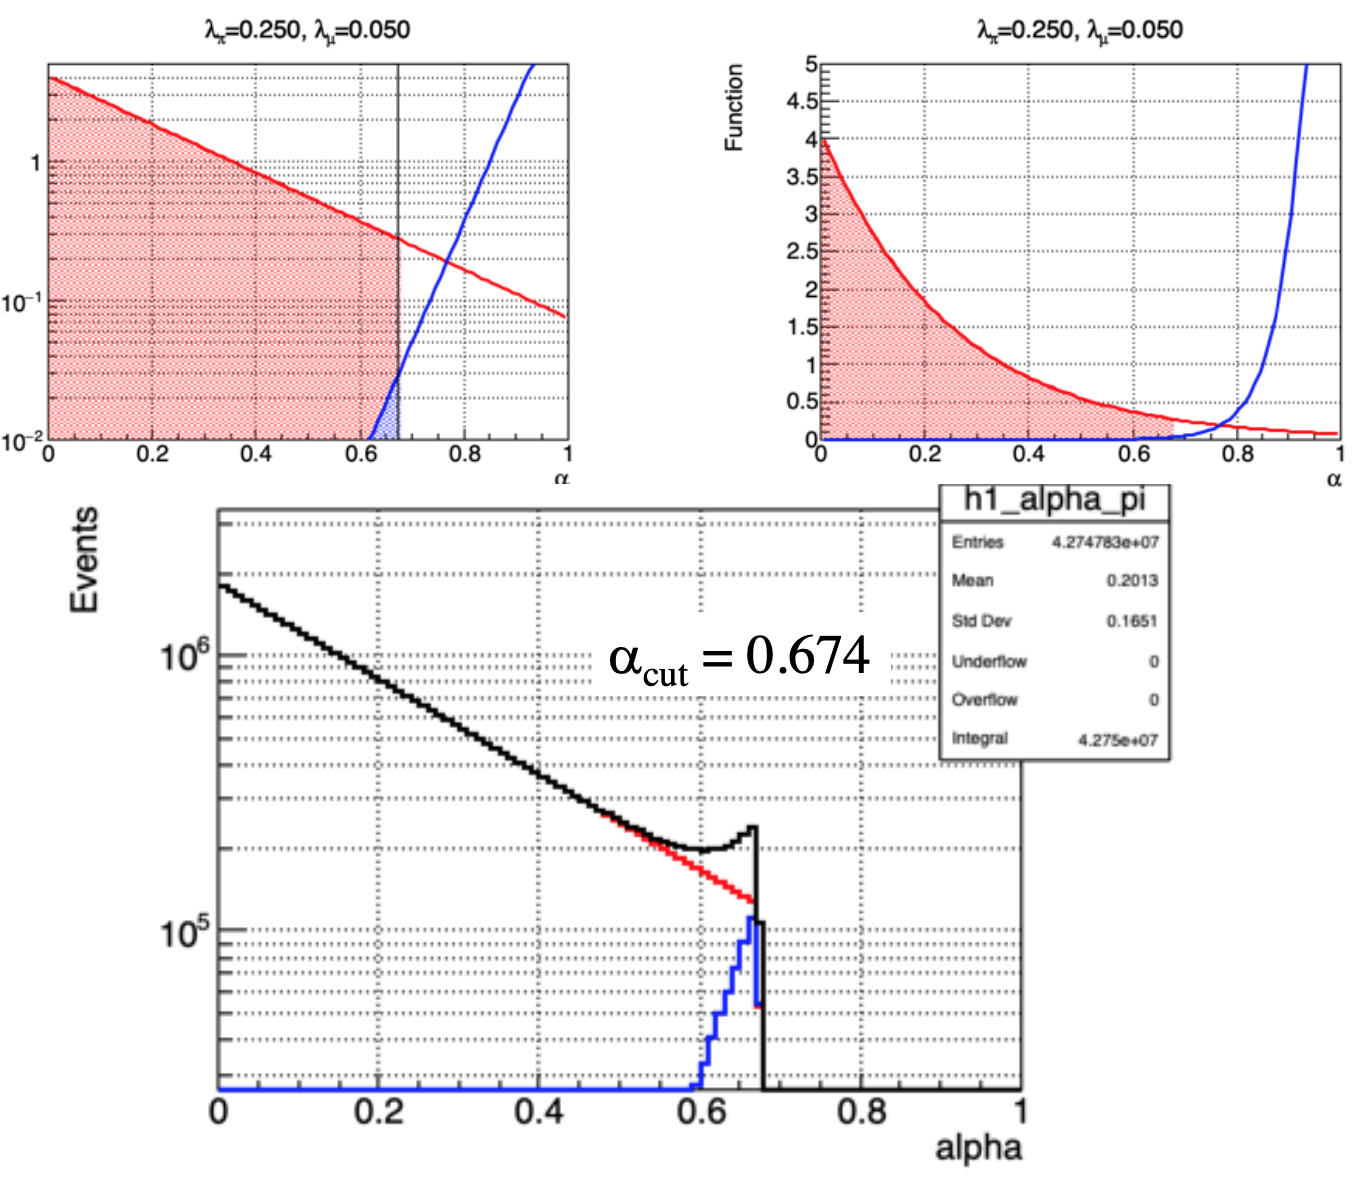
\includegraphics[height=12cm,clip=true]{toy_systematics_c1}
\caption{Toy model for the MVA response. Top Left) Pion function (red), muon function (blue) with a vertical logarithmic scale. 
Top right) Pion function (red) and muon function (blue) with a vertical linear scale.
Bottom) Histogram of the distribution of 25,000 pion and 250,000 muon ``events" generated. Only ``events" below the selection ($\alpha < \alpha_{cut}$) 
are plotted as a function of the randomly distributed MVA response ($\alpha$). The MVA response is taken for $\alpha_{cut}=0.674$. 
The total number of events below the cut is in black, pions in red and muons in blue.
\label{fig:toy_systematics_c1}}
\end{center}
\end{figure} 

\section{Summary}



%\nocite{*}
\bibliographystyle{unsrt}
\bibliography{CPP_PID_systematics}

\end{document}
